% Created 2017-08-22 mar 16:23
\documentclass[letterpaper]{scrartcl}
\usepackage[utf8]{inputenc}
\usepackage[T1]{fontenc}
\usepackage{fixltx2e}
\usepackage{graphicx}
\usepackage{longtable}
\usepackage{float}
\usepackage{wrapfig}
\usepackage{rotating}
\usepackage[normalem]{ulem}
\usepackage{amsmath}
\usepackage{textcomp}
\usepackage{marvosym}
\usepackage{wasysym}
\usepackage{amssymb}
\usepackage{hyperref}
\tolerance=1000
\usepackage{khpreamble}
\usepackage{subfigure}
\author{Kjartan Halvorsen}
\date{}
\title{Bode plot and relative stability exercise}
\hypersetup{
  pdfkeywords={},
  pdfsubject={},
  pdfcreator={Emacs 24.5.1 (Org mode 8.2.10)}}
\begin{document}

\maketitle

\section{Sampling introduces delay}
\label{sec-1}
The continuous-time system 
\[ G(s) = \frac{12}{s(s+2)(s+3)} \]
is sampled using zero-order-hold. The figure below shows the Bode plot and the Nyquist plot for both the continuous-time system (solid lines) and the discrete-time system (dashed lines). 
\begin{center}
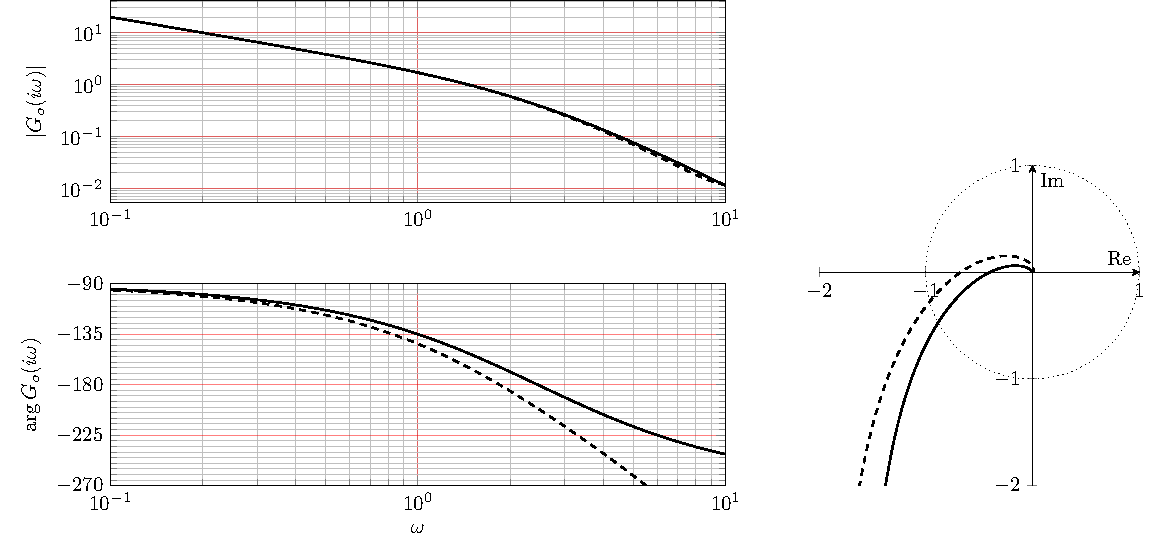
\includegraphics[width=\linewidth]{bode-loop-gain-sol}
\end{center}

\begin{enumerate}
\item Determine the amplitude margins and the phase margins for both systems.
\item What is the delay that the sampling introduces?
\item What is the sampling period?
\end{enumerate}
% Emacs 24.5.1 (Org mode 8.2.10)
\end{document}